\chapter{Statistical Learning Theory and VC-dimension}\label{ch-12}

After the empirical validation techniques, we go back to the
\textbf{analytical estimation} of the expected error (validation error,
for model selection, or test error, for assessment), introduced in
\href{04\%20-\%20Generalizzazione\%20e\%20validazione\%20(introduzione)}{04
- Generalisation and validation (introduction)}. This lecture formally
defines the \textbf{VC-dimension}, computes it for some hypothesis
classes, presents the SLT bound and the principle of \textbf{Structural
Risk Minimization} (SRM), which will lead to SVMs.

Let us recall the alternatives for estimating the error:

\begin{itemize}
\tightlist
\item
  \textbf{analytical}: AIC, BIC (limited to models linear in the
  parameters), MDL, \textbf{SRM with VC-dimension};
\item
  \textbf{by resampling}: cross-validation, bootstrap.
\end{itemize}

\section{The VC-dimension}\label{la-vc-dimension}

To obtain an analytical bound we must evaluate the hypothesis space
\(H\). We need a measure of its \textbf{complexity} (capacity,
expressive power, flexibility) that also works for \textbf{infinite}
\(H\) (such as linear models, with real weights): \(|H|\) therefore
cannot be used. The idea of Vapnik and Chervonenkis is to measure
instead \textbf{the number of distinct instances that \(H\) can
completely discriminate}.

Intuitively, in the case of classification: \emph{how well can \(H\)
discriminate points?} What is the \textbf{maximum number of points that
can be classified correctly, without errors, for all possible
labellings}?

\subsection{Shattering}\label{shattering}

Let \(X\) be the instance space, with \(N\) points (beware: \(N\) here
is the number of instances considered, which may differ from the number
of data \(l\)), and let \(H\) be the hypothesis space for binary
classification.

\begin{itemize}
\tightlist
\item
  There are \(2^N\) possible \textbf{dichotomies} (partitions, or
  labellings of the points with \(-1\) or \(+1\)).
\item
  A dichotomy is \textbf{represented} in \(H\) if there exists a
  hypothesis \(h \in H\) that realises it.
\end{itemize}

\begin{boxdefinition}{Shattering}

\(H\) \textbf{shatters} \(X\) if and only if \(H\) can represent
\textbf{all} possible dichotomies on \(X\) (with zero error): for every
possible labelling of the points there exists a hypothesis \(h \in H\)
consistent with it.

\end{boxdefinition}

\begin{boxexample}{Three points in the plane and lines}

Consider 3 points in \(\mathbb{R}^2\) and as \(H\) the set of lines,
\(h(\mathbf{x}) = \operatorname{sign}(\mathbf{w}^T\mathbf{x} + w_0)\).
A specific dichotomy (for example two points at \(-1\) and one at
\(+1\)) is representable if there exists a line that correctly
separates the points. The possible dichotomies are \(2^3 = 8\).

\end{boxexample}

\begin{figure}[htbp]
\centering
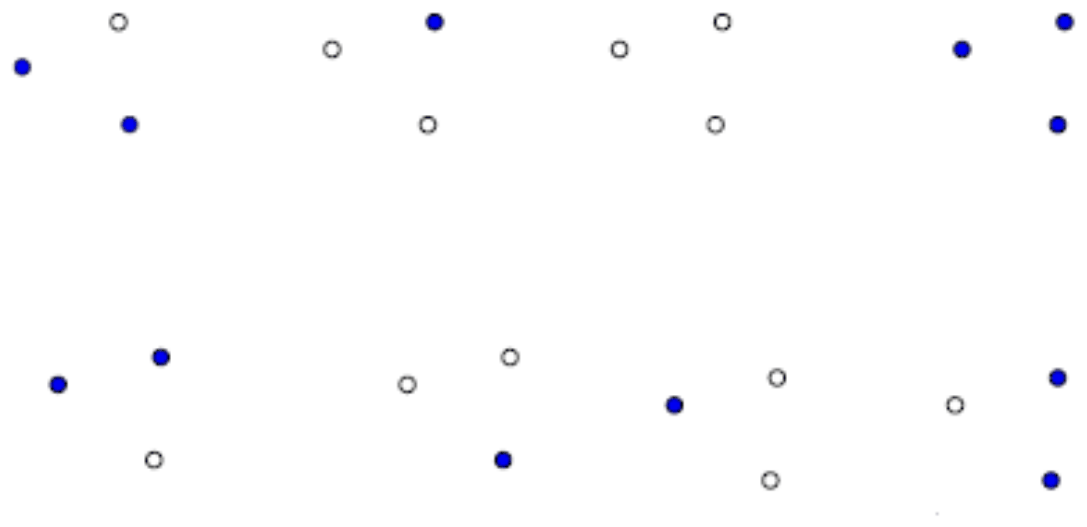
\includegraphics[width=0.71\linewidth,height=0.42\textheight,keepaspectratio]{images/12-slt_dicotomie.png}
\caption{All the \(2^N = 8\) dichotomies of 3 points in
\(\mathbb{R}^2\).}
\end{figure}

\begin{figure}[htbp]
\centering
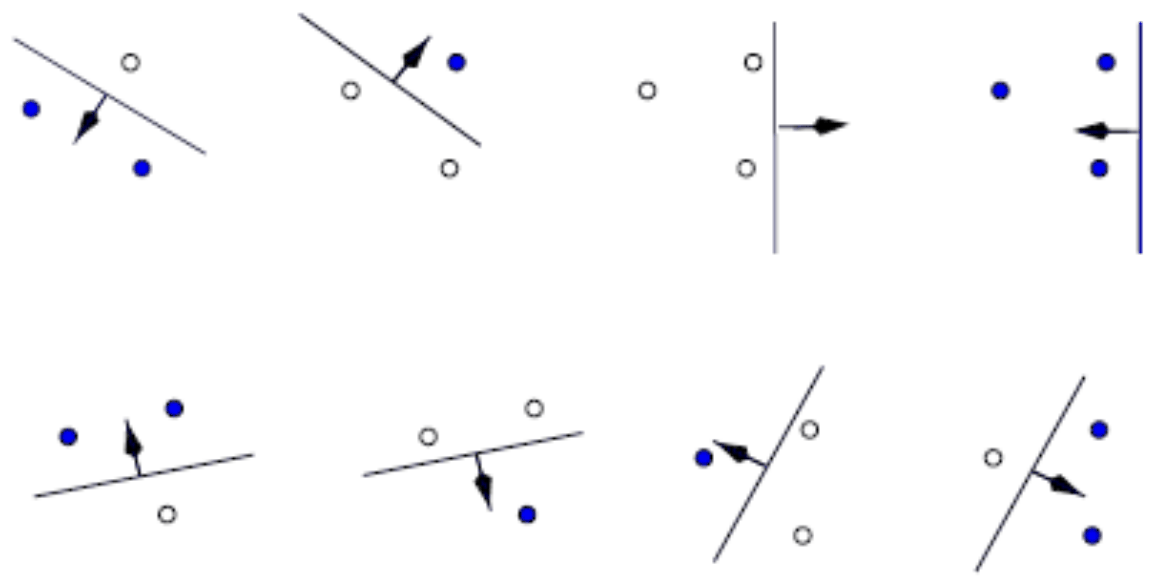
\includegraphics[width=0.71\linewidth,height=0.42\textheight,keepaspectratio]{images/12-slt_shattering.png}
\caption{For each dichotomy there is a separating line: linear functions
shatter these 3 points.}
\end{figure}

\subsection{Definition of
VC-dimension}\label{definizione-di-vc-dimension}

\begin{boxdefinition}{VC-dimension}

The \textbf{VC-dimension} of a class of functions \(H\) is the
\textbf{maximum cardinality of a set of points} (in some configuration)
of \(X\) that can be shattered by \(H\). \(VC(H) = p\) means that:

\begin{itemize}
\tightlist
\item
  \(H\) shatters \textbf{at least one} set (configuration) of \(p\)
  points;
\item
  \(H\) does \textbf{not} shatter \textbf{any} set of \(p+1\) points.
\end{itemize}

If sets of arbitrarily large size can be shattered,
\(VC(H) = \infty\).

\end{boxdefinition}

Note the asymmetry: for the lower bound \textbf{one} shatterable
configuration is enough; for the upper bound one must show that
\textbf{no} configuration of \(p+1\) points is shatterable.

\subsection{VC-dimension of hyperplanes in the
plane}\label{vc-dimension-degli-iperpiani-nel-piano}

\begin{itemize}
\tightlist
\item
  \textbf{\(VC(H) \ge 3\)}: we have just shown it with 3 non-collinear
  points. Not all configurations of 3 points are shatterable: three
  \textbf{collinear} points with the middle one of a different class
  are not linearly separable. But \textbf{one} shatterable
  configuration is enough.
\item
  \textbf{\(VC(H) < 4\)}: given any 4 points in the plane, one can
  always draw the 6 segments connecting them in pairs, and two of these
  cross (if the 4 points form a convex quadrilateral they are the
  diagonals; if one is inside the triangle of the others, the labelling
  with the inner point of a different class is chosen). Putting in the
  same class the points connected by the crossing segments, they cannot
  be separated linearly: it is \textbf{XOR}.
\end{itemize}

\begin{figure}[htbp]
\centering
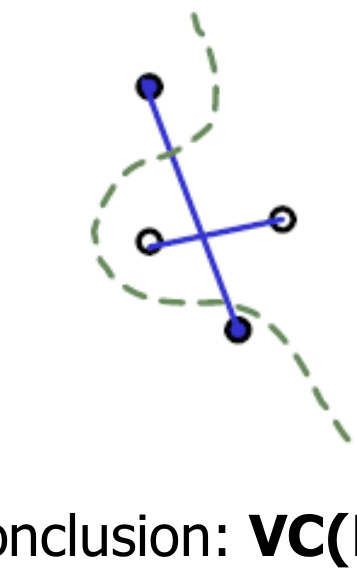
\includegraphics[width=0.31\linewidth,height=0.42\textheight,keepaspectratio]{images/12-slt_quattro-punti.png}
\caption{With 4 points there is always an XOR-like labelling that cannot
be separated by a line.}
\end{figure}

Conclusion: \textbf{\(VC(H) = 3\)} for hyperplanes (LTU) in
\(\mathbb{R}^2\).

\begin{boxtheorem}{VC-dimension of hyperplanes}

The VC-dimension of the class of separating hyperplanes (LTU) in an
\(n\)-dimensional space is \(n + 1\).

\end{boxtheorem}

It is an upper bound: constraining the model (for example by bounding
the norm of the weights, as will be seen in SVMs) it can decrease.

\subsection{Other examples}\label{altri-esempi}

{\def\LTcaptype{none} % do not increment counter
\begin{longtable}[]{@{}
  >{\raggedright\arraybackslash}p{(\linewidth - 2\tabcolsep) * \real{0.5000}}
  >{\raggedright\arraybackslash}p{(\linewidth - 2\tabcolsep) * \real{0.5000}}@{}}
\toprule\noalign{}
\begin{minipage}[b]{\linewidth}\raggedright
Class \(H\)
\end{minipage} & \begin{minipage}[b]{\linewidth}\raggedright
VC-dim
\end{minipage} \\
\midrule\noalign{}
\endhead
\bottomrule\noalign{}
\endlastfoot
Lines in \(\mathbb{R}\) (thresholds, \(\operatorname{sign}(w_1x + w_0)\))
& 2 \\
Intervals on \(\mathbb{R}\) & 2 \\
Circles centred at the origin in 2D,
\(\operatorname{sign}(\mathbf{x}\cdot\mathbf{x} - b)\) & 1 \\
Circles centred at the origin,
\(\operatorname{sign}(k\,\mathbf{x}\cdot\mathbf{x} - b)\) & 2 \\
Circles (free radius and centre) in 2D & 3 \\
Circles (fixed radius, free centre) in 2D & 3 \\
\end{longtable}
}

(For circles centred at the origin with a single parameter \(b\), the
circle includes points close to the origin: with two points at
different distances one cannot label ``+'' the farther one and ``−''
the closer one. Adding \(k\) allows inside and outside to be swapped,
and the VC-dim rises to 2.)

The VC-dimension can be hard to compute for models with non-linear
parameters.

\subsection{VC-dimension and number of
parameters}\label{vc-dimension-e-numero-di-parametri}

Is the VC-dimension the number of free parameters? \textbf{They are
related but do not coincide}:

\begin{itemize}
\tightlist
\item
  in the circle example, classes with the \textbf{same} number of
  parameters have different VC-dims, and vice versa;
\item
  \textbf{redundant} parameters can be added without changing
  anything;
\item
  there are models with \textbf{a single parameter and infinite
  VC-dim} (the classic example is \(\operatorname{sign}(\sin(\alpha x))\),
  which with a large enough \(\alpha\) shatters any suitably chosen set
  of points);
\item
  for the \textbf{nearest neighbor} the VC-dim is \textbf{infinite}
  (1-NN correctly classifies any labelling of the training set).
\end{itemize}

\section{The analytical risk
bound}\label{il-bound-analitico-sul-rischio}

Let \(N\) be the number of data (\(l\)).

\begin{boxtheorem}{VC-bound}

With probability at least \(1 - \delta\), for every \(h \in H\) (with
\(VC < N\)): \[
R[h] \;\le\; R_{emp}[h] + \varepsilon(VC, N, \delta),
\] where the right-hand side is the \textbf{guaranteed risk} and
\(\varepsilon\) is the \textbf{VC-confidence}. For example, for the 0/1
loss: \[
\varepsilon(VC, N, \delta) = \sqrt{\frac{VC\left(\ln\frac{2N}{VC} + 1\right) - \ln\frac{\delta}{4}}{N}}.
\]

\end{boxtheorem}

There are different formulations for different function classes and
tasks. The interpretation is the one already seen:
\(\varepsilon \to 0\) as \(N\) grows, \(\varepsilon\) grows with the
VC-dim, and the bound on \(R\) has a U-shaped trend as the VC-dim
grows.

The formula shows it clearly: \(\varepsilon\) depends essentially on
the ratio \(VC/N\) (up to logarithms). Doubling the data has the same
effect as halving the complexity.

The bound makes it possible to \textbf{estimate the error on future
data} based only on the training error and on the VC-dimension of
\(H\), and the VC-confidence can be computed \textbf{before} learning.

\begin{boxwarning}{``Worst case'' bound}

The resulting bounds are \emph{worst case}: they must hold for all
functions and all training sets, except a fraction \(\delta\). This is
why they are often very loose.

\end{boxwarning}

\begin{boxtip}{A practical consequence}

For many reasonable classes (e.g.\ linear approximators) the VC-dim is
\textbf{linear in the number of free parameters}. Therefore, to learn
``well'', a number of examples \textbf{linear in the VC-dimension} is
needed (and hence, in this case, in the number of parameters). It is a
theoretical explanation of practical heuristics such as ``at least
\(k\) examples per parameter are needed''.

\end{boxtip}

\section{Structural Risk
Minimization}\label{structural-risk-minimization}

\textbf{SRM} uses the VC-dimension as a control parameter to minimise
the risk bound. Assuming finite VC-dims, a \textbf{nested structure} of
hypothesis spaces ordered by VC-dim is defined: \[
H_1 \subseteq H_2 \subseteq \dots \subseteq H_n, \qquad VC(H_1) \le \dots \le VC(H_n).
\]

Examples of structures:

\begin{itemize}
\tightlist
\item
  neural networks with an increasing number of \textbf{hidden units}
  (roughly), but also with an increasing number of \textbf{epochs} (we
  know that the size of the weights also matters: the network is a
  variable-dimension space);
\item
  polynomials of increasing \textbf{degree} \(M\);
\item
  increasing values of \(c\), where \(\|\mathbf{w}\| < c\) for
  \textbf{regularisation} (or equivalently controlled by \(\lambda\));
\item
  decision trees with an increasing number of nodes (roughly).
\end{itemize}

The \textbf{important hyperparameters} are precisely those related to
the VC-dimension.

\subsection{SRM for model
selection}\label{srm-per-la-model-selection}

As the VC-dim grows, the empirical (training) error \textbf{decreases}
and the VC-confidence \textbf{increases}. SRM looks for the trade-off
on the bound \[
R \le R_{emp} + \varepsilon(1/l, VC, 1/\delta),
\] i.e.\ it chooses the model \(h\) with the \textbf{best bound on the
true risk}.

\begin{figure}[htbp]
\centering
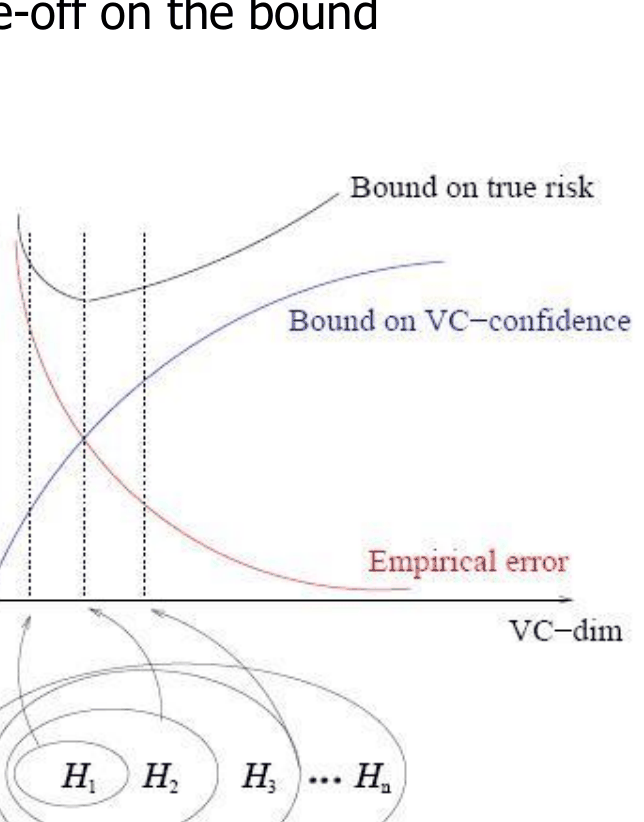
\includegraphics[width=0.46\linewidth,height=0.42\textheight,keepaspectratio]{images/12-slt_srm.png}
\caption{Structural Risk Minimization: on a nested structure of
hypothesis spaces, the one that minimises the risk bound is chosen.}
\end{figure}

\begin{figure}[htbp]
\centering
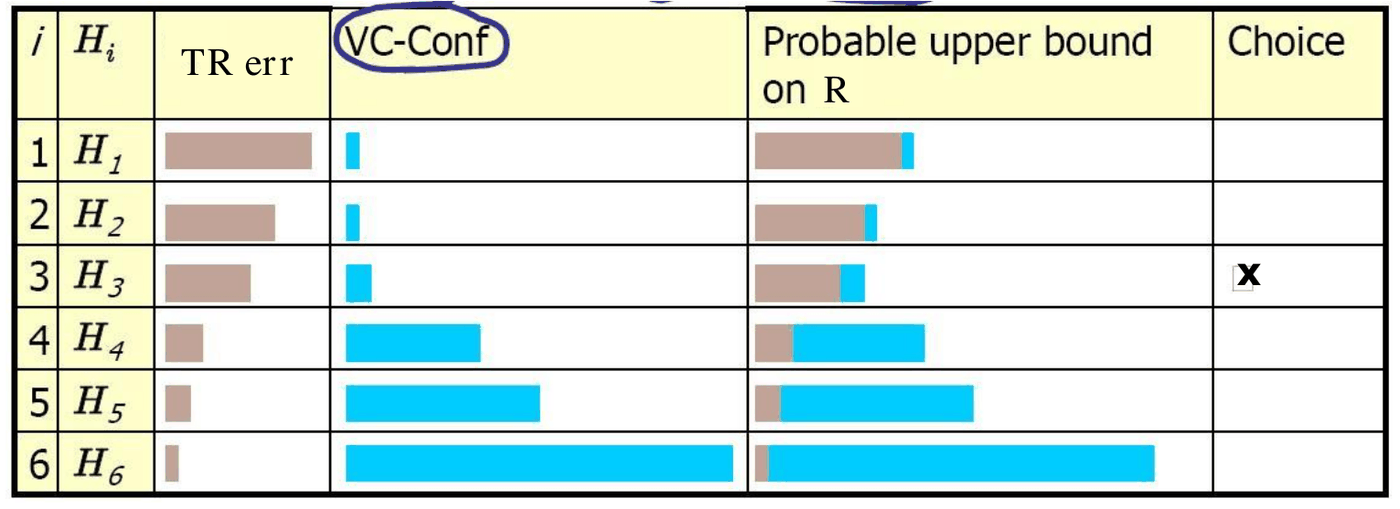
\includegraphics[width=0.86\linewidth,height=0.42\textheight,keepaspectratio]{images/12-slt_srm-tabella.png}
\caption{Model selection with SRM: \(H_3\) is chosen, with the minimum
probable bound on \(R\).}
\end{figure}

\begin{boxwarning}{Warning}

The VC-confidence can be \textbf{very conservative}: even hundreds of
times larger than the overfitting effect observed empirically.

\end{boxwarning}

\subsection{What the bound is for}\label{a-cosa-serve-il-bound}

\begin{itemize}
\tightlist
\item
  It provides a \textbf{theoretical foundation} for principled ML,
  independent of the details of the model or algorithm; it highlights
  the role of \textbf{complexity control}; it shows that the optimal
  choice of complexity (on the structure) minimises the expected risk:
  this is the \textbf{inductive principle of SRM}.
\item
  As an \textbf{estimate of the predictive error} it is rarely used:

  \begin{itemize}
  \tightlist
  \item
    it can be very loose, but it remains useful for \textbf{model
    selection}, where the \textbf{relative size} (the \emph{ranking})
    of the errors matters;
  \item
    it is a probabilistic upper bound valid for \textbf{all} functions
    in the class, so one can search within the class;
  \item
    it is hard to compute the VC-dim of specific classes;
  \item
    the raw bound (too pessimistic) may not be adequate for a reliable
    evaluation of the generalisation error (\textbf{model assessment});
    tighter bounds are being developed.
  \end{itemize}
\item
  It indicates a direction for developing \textbf{new models} guided by
  SRM, towards principled approaches rather than empirical trial and
  error.
\end{itemize}

\subsection{Two practical approaches to
SRM}\label{due-approcci-pratici-alla-srm}

\begin{enumerate}
\def\labelenumi{\arabic{enumi}.}
\tightlist
\item
  \textbf{Fix the structure/complexity} (and hence the VC-confidence)
  and \textbf{minimise the training error}. It can be used with neural
  networks. Training heuristics may already implement an
  \textbf{implicit} SRM (early stopping, \ldots); or SRM is implemented
  with \textbf{Tikhonov regularisation}, minimising a loss \(R_{emp}\)
  + complexity term, which considers both terms.
\item
  \textbf{Fix the training error} and \textbf{automatically minimise
  the VC-confidence}. How? This is the idea of \textbf{SVMs}
  (\href{13\%20-\%20Support\%20Vector\%20Machines}{13 - Support Vector
  Machines}).
\end{enumerate}

\begin{boxabstract}{Summary}

The \textbf{VC-dimension} measures the capacity of \(H\) as the maximum
number of points that \(H\) can shatter (classify correctly for every
labelling). For hyperplanes in \(\mathbb{R}^n\) it is \(n+1\); it does
not coincide with the number of parameters (it can be infinite with a
single parameter, and it is infinite for NN). The \textbf{VC-bound}
\(R \le R_{emp} + \varepsilon(VC, N, \delta)\) links risk, training
error, complexity and number of data. \textbf{SRM} chooses, in a nested
structure of spaces, the one that minimises the bound. The bounds are
often loose, but they provide the theoretical foundation of complexity
control.

\end{boxabstract}

\begin{boxquestion}{Possible exam questions}

\begin{itemize}
\tightlist
\item
  Define shattering and VC-dimension.
\item
  Prove that the VC-dim of lines in the plane is 3.
\item
  Does the VC-dim coincide with the number of free parameters?
  Examples.
\item
  Write the VC-bound and interpret its terms.
\item
  What is Structural Risk Minimization? Examples of nested structures.
\item
  What are the practical limits of the bound? What is it useful for
  anyway?
\end{itemize}

\end{boxquestion}
